\chapter{Label-free high-throughput cell screening}

Flow cytometry is a powerful tool for cell counting and biomarker detection in biotechnology and medicine especially with regards to blood analysis. Standard flow cytometers perform cell type classification both by estimating size and granularity of cells using forward- and side-scattered light signals and through the collection of emission spectra of fluorescently-labeled cells. However, cell surface labeling as a means of marking cells is often undesirable as many reagents negatively impact cellular viability or provide activating/inhibitory signals, which can alter the behavior of the desired cellular subtypes for downstream applications or analysis. To eliminate the need for labeling, we introduce a label-free imaging-based flow cytometer that measures size and cell protein concentration simultaneously either as a stand-alone instrument or as an add-on to conventional flow cytometers. Cell protein concentration adds a parameter to cell classification, which improves the specificity and sensitivity of flow cytometers without the requirement of cell labeling. This system uses coherent dispersive Fourier transform to perform phase imaging at flow speeds as high as a few meters per second.

\section{Introduction}

Cell protein content measurement can be used in many biomedical applications such as blood doping detection \cite{grover2011measuring}, infection monitoring \cite{mrema1979concentration}, drug development and screening \cite{chun2012rapidly}, studies of necrosis and apoptosis \cite{martin1990hl,wyllie1982hormone}, cell cycle progression and differentiation \cite{wolff1972separation,maric1998buoyant,bista2011quantification}, and in cancer diagnostics \cite{bosslet1981rapid,phillips2012quantification,phillips2012optical}. Current methods for cell protein concentration measurement include electrical methods based on dielectrophoresis \cite{gupta2012apostream}, mechanical methods based on microchannel cantilevers \cite{grover2011measuring}, and optical methods based on scattering patterns \cite{tycko1985flow}, emission spectra of external cavity lasers \cite{liang2007determining}, and holographic and phase microscopy \cite{rappaz2005measurement,curl2005refractive,lue2009live,gorthi2012phase}. These methods are either inherently too slow for high-speed flow cytometry applications or require feedback mechanisms \cite{popescu2006optical} to provide necessary precision. Furthermore, size-based classification can also be used for label-free identification of cells of interest in a suspension stream \cite{vona2000isolation}. However, due to significant overlap of size ranges between most mammalian cells, size-based technologies require additional layers of parametric gating to be useful as a diagnostic tool \cite{di2013hyperspectral}.  It is known that the refractive index of a cell is proportional to its protein content \cite{barer1954refractometry}. As such, the simultaneous measurement of refractive index and size of cells would be predicted to provide two independent parameters for cell classification.

In this chapter, we propose a fast and high-precision optical cell density and size measurement method based on serial time-encoded amplified microscopy (STEAM) \cite{goda2009serial}. STEAM is a continuous imaging technique that captures tens of million frames-per-second with sub-nanosecond shutter speed. However, earlier versions of STEAM were dependent on cell labeling due to low intensity contrast of individual cells \cite{goda2012high}. Here, we introduce a new configuration of STEAM capable of high-speed phase microscopy and demonstrating label-free single-cell classification and diagnostics. In addition, we demonstrate a new design of STEAM that minimizes loss and chromatic aberration, decreases polarization sensitivity, and results in a smaller footprint \cite{fard2011nomarski}. In contrast to previous implementations of STEAM, which were based on refractive optics, the new design employs reflective optics.

The basic principle of STEAM involves two steps both performed optically. In the first step, the spectrum of a broadband optical pulse is converted by a spatial disperser into a rainbow that illuminates the target. Therefore, the spatial information (image) of the object is encoded into the spectrum of the resultant reflected or transmitted rainbow pulse. A 1D rainbow is used in flow imaging as the flow causes the cell to be scanned in the second dimension. In the second step, the spectrum of the image-encoded pulse is mapped into a serial temporal signal that is stretched in time to slow it down such that it can be digitized in real-time \cite{goda2013dispersive}. This optically-amplified time-stretched serial stream is detected by a single-pixel photodetector and the image is reconstructed in the digital domain. Subsequent pulses capture repetitive frames, hence the laser pulse repetition rate corresponds to the frame rate of STEAM and the shutter speed (exposure time) corresponds to the temporal width of the pulse. The key innovations in STEAM that enable high speed real-time imaging are photonic time stretch for digitizing fast images in real-time and the optical image amplification for compensating the low number of photons collected during the ultra-short shutter time.

The contrast limitations of label-free single-cell imaging of STEAM led us to develop a derivative of STEAM, referred to as Coherent-STEAM, to capture phase images of cells in flow. We use a Michelson interferometer to map the phase image of cells into the spectrum of broadband optical pulses. This phase imaging technique exploits the fast shutter speed of STEAM to freeze path length fluctuations of interferometer arms and attains nanometer phase resolution with no need for feedback stabilization of the interferometer \cite{mahjoubfar2011high,goda2012hybrid,mahjoubfar20133d}. We use Coherent-STEAM to measure the refractive index of individual cells in an imaging flow cytometer by simultaneous measurement of size and total optical phase-shift induced by the cells. As an example, we use our label-free STEAM-based cell classifier to distinguish OT-II T cell hybridoma from SW480 epithelium cancer cells. We show that adding protein concentration to size as an additional classification parameter increases accuracy and specificity in flow cytometry.

\section{Experimental setup}

A mode-locked fiber laser generates pulses at 1565 nm with a repetition rate of 36.128 MHz and a pulse width slightly less than 100 fs (Figure Figure \ref{fig:BOE2013_Figure1}). Pulses are spectrally broadened with a highly nonlinear fiber to approximately 100 nm bandwidth \cite{boyraz2000broadband}. A short dispersion compensating fiber with an overall dispersion of 60 ps/nm is used to temporally broaden pulses to 1.2 ns, so an erbium doped fiber amplifier (EDFA) can amplify them without any distortion. Amplified pulses enter a coarse wavelength division multiplexing (WDM) filter, and the output of 1591 nm channel is used to shape laser pulses with a considerably flat spectrum over 1581 nm to 1601 nm bandwidth. These pulses pass through an optical circulator and are coupled to free-space with a fiber collimator.

\begin{figure}[htb!]
\centering
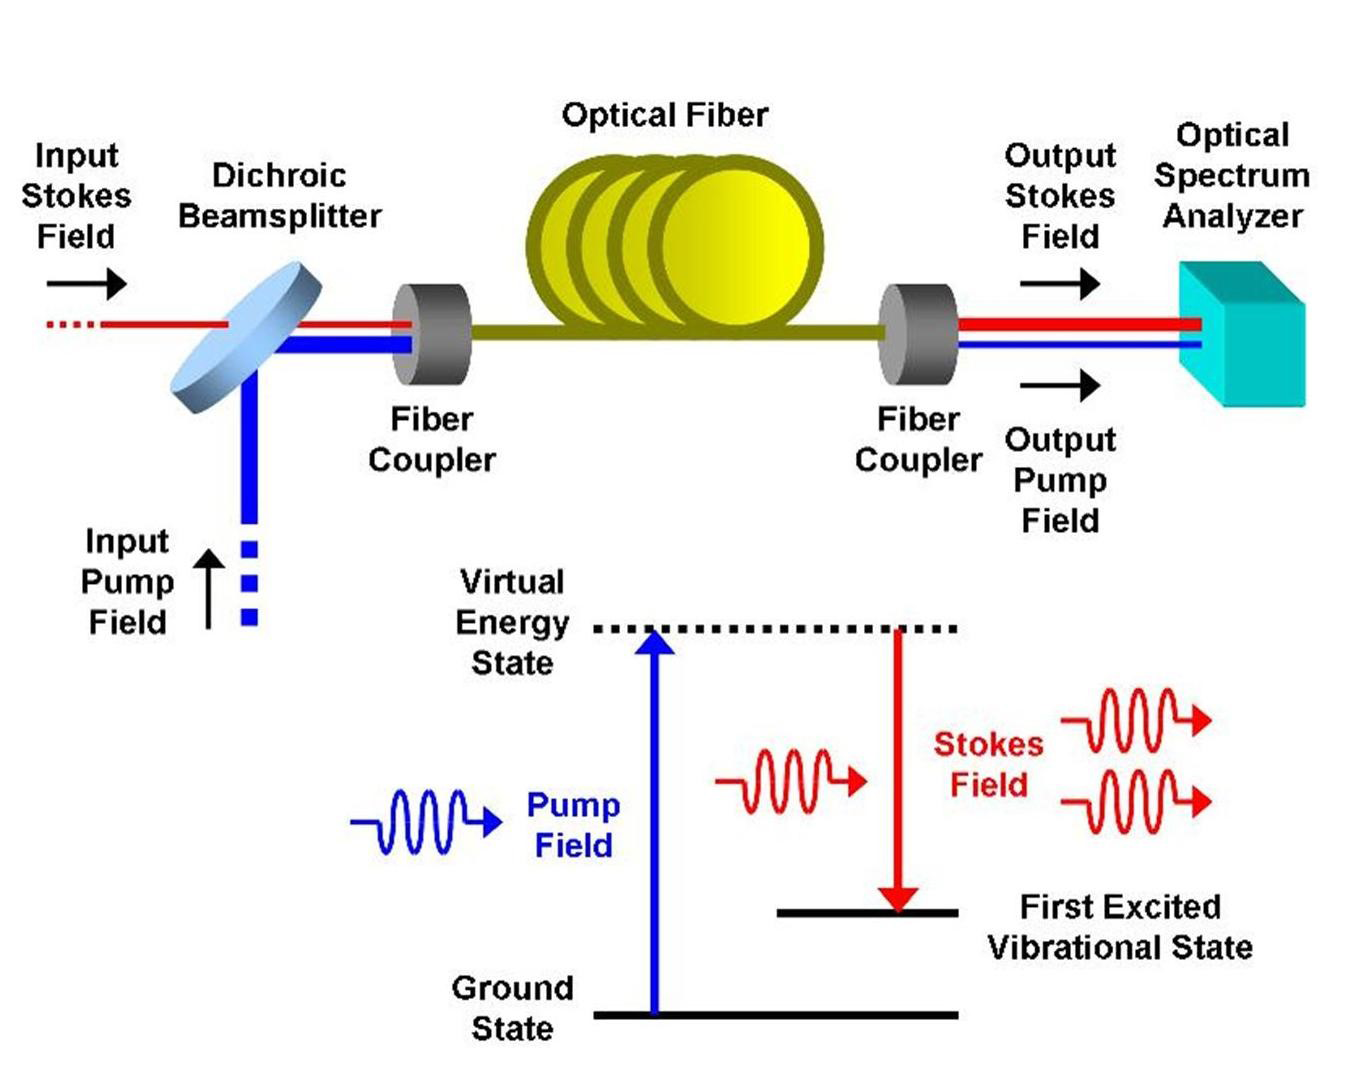
\includegraphics[scale=1]{BOE2013/Figure1.png}
\caption{Optical setup of Coherent-STEAM. A Coherent-STEAM setup is formed by combination of STEAM and a Michelson interferometer. A pair of diffraction gratings generates a 1D rainbow with different wavelength components imaging different points on the cells flowing in a microfluidic channel. A pellicle beam-splitter and two identical long working-distance objective lenses are used to form the interferometer for phase measurement. Back apertures of objective lenses are fully illuminated with each wavelength component of the broadband mode-locked laser pulses to ensure diffraction-limited resolution. An amplified time-stretch system chirps, stretches, and amplifies each pulse, so that different wavelength components reach the photodetector serially. A very shallow microfluidic channel with hydrodynamic focusing is designed and fabricated to align cells within the focal depth of the system.}
\label{fig:BOE2013_Figure1}
\end{figure}

Free-space laser pulses are linearly polarized with quarter- and half-wave plates, and then they are spatially dispersed with a pair of reflection diffraction gratings, so that each wavelength component of the collimated beam is positioned at a different lateral point similar to a rainbow. A pair of 90 degree off-axis parabolic gold-coated mirrors with 152.4 mm and 25.4 mm reflected focal lengths are used to form a beam reducer that shrinks the rainbow beam 6 times. Parabolic gold-coated mirrors are used to minimize loss, aberration, and polarization sensitivity. In addition, a 15 degree off-axis parabolic gold-coated mirror with 635 mm reflected focal length and a 0.4 numerical aperture long working-distance objective lens further shrink the rainbow to about 130 μm field of view. Using reflective optics, we managed to improve the signal-to-noise ratio by about 9 dB. A beam splitter is used to form two arms of a Michelson interferometer. Different wavelength components of the rainbow are focused on a mirror in the reference arm and on the reflective substrate of a microfluidic device in the sample arm. Cells hydrodynamically focused at the center of the channel flow at a velocity of 1.3 m/s. The rainbow pulses pass through the cells and are reflected back by the mirror substrate of the microfluidic device. The total bandwidth of the pulses interrogating the cells in our Coherent STEAM is less than 20 nm centered at 1590 nm, giving a negligible fractional bandwidth of 1.3\%. Therefore, the color-dependency of absorption is very small and can be easily neglected. The reflected pulses from the microfluidic device and reference mirror interfere at the beam splitter and return to the fiber, where they are directed with the optical circulator to an amplified time-stretch system.

The amplified time-stretch system is a combination of a Raman amplifier and a dispersive fiber to perform dispersive Fourier transform \cite{goda2013dispersive}. Four Raman pump lasers at 1450 nm, 1470 nm, 1490 nm, and 1505 nm are used to amplify the signal for about 15 dB over the whole optical bandwidth uniformly. The dispersive fiber chirps and stretches each pulse in time to about 27 ns. So, different wavelength components reach the photodetector serially. An analog-to-digital convertor (ADC) with a sampling rate of 50 GSps and 20 GHz bandwidth is used to acquire the output signal of the photodetector.

The photodetector output signal, $I(t)$, is digitized and recorded by the ADC (Figure \ref{fig:BOE2013_Figure2}a). This signal shows sequential laser pulses. Each pulse is used to form one line image. Therefore, the boundaries of pulses are determined precisely, and each pulse is saved separately as a frame for further processing (Figure \ref{fig:BOE2013_Figure2}b). The analytic form of each pulse is generated using Hilbert transformation after the low frequency components corresponding to intensity variations are filtered out \cite{ikeda2005hilbert}. The phase component of this analytic form is extracted, while its amplitude component is discarded (Figure \ref{fig:BOE2013_Figure2}c). Because the phase varies over a wide range (much larger than $2 \pi$ radians), it shows unrealistic discontinuities. An unwrapping algorithm is used to fix these discontinuities, and the result shows an approximately linear phase increase over the time for each pulse or frame (Figure \ref{fig:BOE2013_Figure2}d). The unwrapping algorithm adds multiples of $\pm 2 \pi$ to make the absolute jumps between consecutive samples in a frame smaller than $\pi$ radians when they are greater than $\pi$ radians. If the linear component of the phase, which corresponds to the fringe (modulation) frequency, $f_m$, due to the interferometer arms’ length mismatch, and the background phase level, $\varphi_0$, are subtracted, the phase shift induced by the cells in the optical pulse can be observed (Figure \ref{fig:BOE2013_Figure2}e); i.e. 
\begin{equation}
\Delta\varphi(t)= unwrap(\arg(I_{BP}(t)+j \cdot \hat{I}_{BP}(t))) - 2 \pi f_m t - \varphi_0
\end{equation}
in which $I_{BP}(t)$ is a band-pass filtered form of $I(t)$ with only spectral features modulated at $f_m$, and $\hat{I}_{BP}(t)$ is the Hilbert transform of $I_{BP}(t)$. Many phase line images generated from subsequent frames are combined to form a spatial map of optical path difference (OPD) in two dimensions (Figure \ref{fig:BOE2013_Figure2}f). Since we know the mapping of space to time from the rainbow characteristics and flow speed, OPD at each point is calculated as
\begin{equation}
OPD(x,y) = \frac{\lambda(x)}{2 \pi} \Delta\varphi(x,y)
\end{equation}
where $x$ and $y$ are coordinates in the rainbow and flow directions, respectively; $\lambda(x)$ is the wavelength at position $x$ along the rainbow; and $\Delta\varphi(x,y)$ is the phase shift induced by the cell at point $(x,y)$.

\begin{figure}[htb!]
\centering
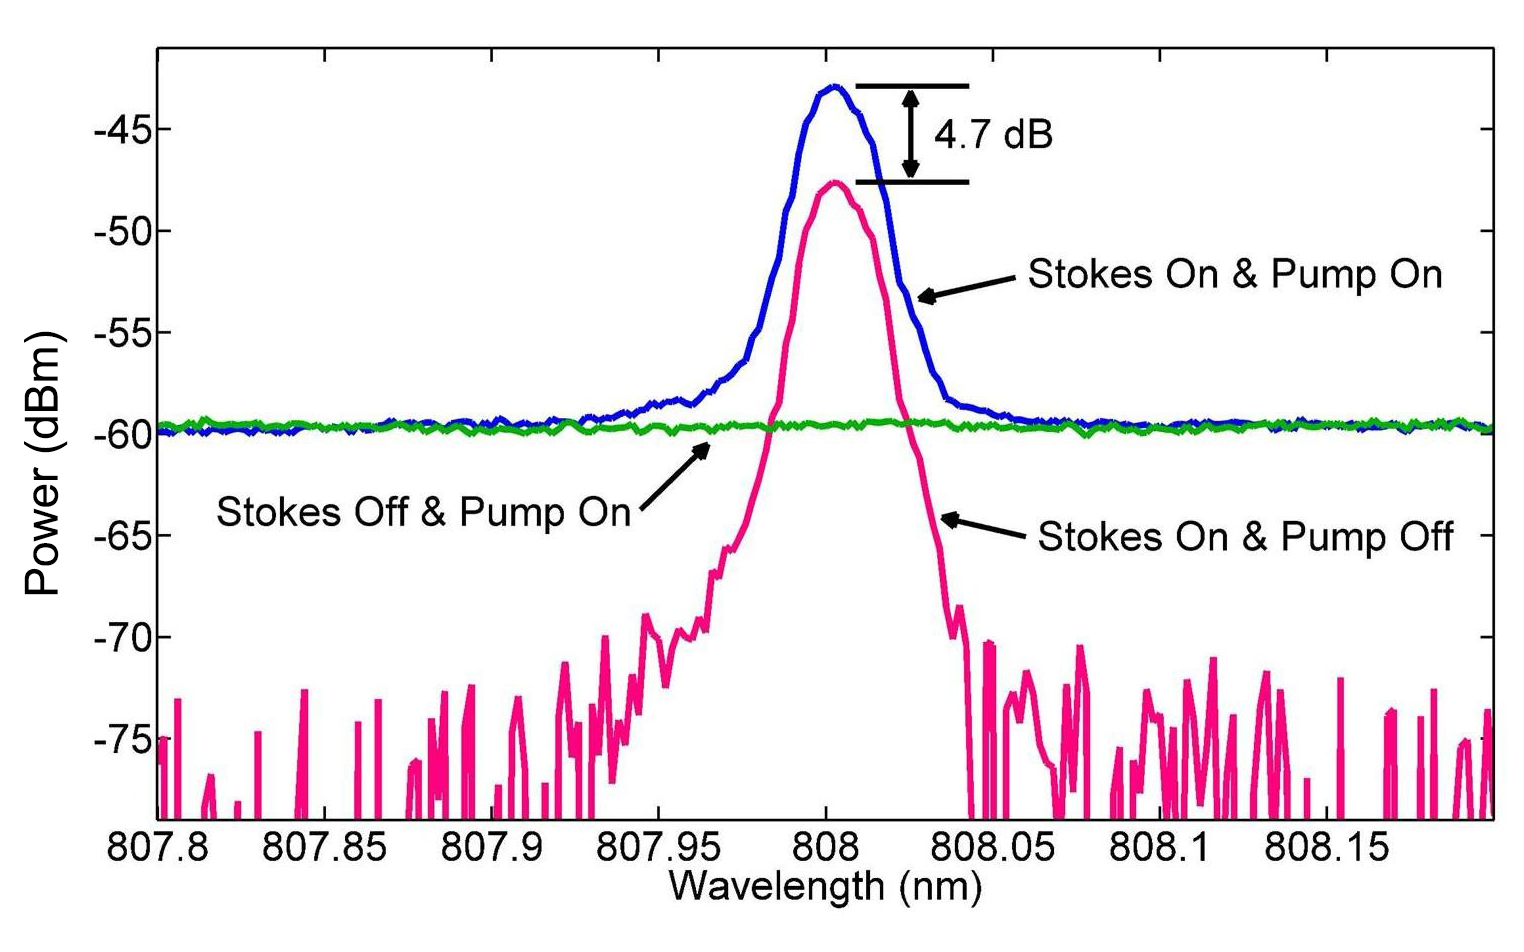
\includegraphics[scale=1]{BOE2013/Figure2.png}
\caption{Digital signal processing of Coherent-STEAM. (a) The photodetector output signal is digitized and recorded by an ADC. This signal shows sequential laser pulses. (b) Each pulse is saved separately as a frame for further processing. (c) The analytic form of high-frequency components of each pulse is generated using Hilbert transformation, and the phase component of this analytic form is extracted. (d) An unwrapping algorithm is used to fix unrealistic phase jumps, and the result shows an approximately linear phase increase. (e) If the phase component of the interferometer fringe frequency is removed, the phase induced by cells in optical pulse can be seen. (f) Many of these line images generated from subsequent frames are used to form a spatial map of optical path difference in two dimensions, which is used for cell characterization.}
\label{fig:BOE2013_Figure2}
\end{figure}

Spatial map of optical path difference can be used to extract the refractive index contrast between the cell and the surrounding liquid.  If the thickness of the cell at point $(x,y)$ is $t(x,y)$,
\begin{equation}
OPD(x,y) = 2 \Delta n_{cell} \cdot t(x,y)
\label{eqn:BOE2013_Equation3}
\end{equation}
where $\Delta n_{cell} = n_{cell} - n_{liquid}$ in which $n_{cell}$ and $n_{liquid}$ are the refractive indices of the cell and the surrounding liquid, respectively. The factor 2 is to account for the fact that each wavelength component passes the cell twice in Michelson interferometer. If we integrate Equation \eqref{eqn:BOE2013_Equation3} over the area of the cell, we can derive an average refractive index contrast, which corresponds to protein concentration of the cell:
\begin{equation}
\Delta n_{cell} = \frac{\iint_{cell} OPD(x,y) \ud x \ud y}{2V_{cell}}
\label{eqn:BOE2013_Equation4}
\end{equation}
where $V_{cell} = \iint_{cell} t(x,y) \ud x \ud y$ is the volume of the cell. Most of the cells relax to a spherical shape when they are released from substrates and brought into suspension \cite{revel1974adhesion,whur1977substrate}. Therefore, if we know the diameter of the cell, $d_{cell}$, we can estimate its volume as $V_{cell} \approx \pi d_{cell}^3/6$.

\section{Results and discussion}
Spherical polystyrene beads with a NIST traceable diameter of 5 μm are used to calibrate the image processing algorithm for size measurements. A custom designed algorithm in CellProfiler software \cite{carpenter2006cellprofiler} is used to detect the beads or cells in spatial map of optical path difference (Figure \ref{fig:BOE2013_Figure3}). Bead or cell diameter is measured along the rainbow direction to eliminate size measurement inaccuracies caused by fluctuations of flow speed (Figure \ref{fig:BOE2013_Figure3}a). Due to limited optical resolution of the setup, the bead or cell edges are blurred, generating a small phase signal outside of the diameter bars. The diameter along the rainbow direction is equal to the diameter along the interrogation optical beam for spherical-shape beads or cells in suspension, including the samples in our experiments. 

\begin{figure}[htb!]
\centering
\includegraphics[scale=1]{BOE2013/Figure3.png}
\caption{Calibration with NIST traceable beads. Polystyrene beads with a NIST traceable diameter of 5 μm are used to calibrate the image processing algorithm for size measurements. (a) A custom designed image processing algorithm in CellProfiler software is used to find the beads in spatial map of optical path difference and measure the diameter. (b) Histogram of bead diameters demonstrates the measured size distribution has an expected mean of 5 µm and a standard deviation within the range of optical resolution limit. (c) Since all the beads are made out of the same material, the coefficient of variation for refractive indices ($0.014/1.57 = 0.89\%$) is much smaller than that of diameters ($0.405/5.06 = 8.00\%$).}
\label{fig:BOE2013_Figure3}
\end{figure}

Histogram analysis of bead diameter distribution for more than one hundred beads with corresponding Gaussian fit to measurements demonstrates that the measured size distribution has a standard deviation of 0.4 μm and an expected mean of 5 μm (Figure \ref{fig:BOE2013_Figure3}b). The broadening in the distribution is caused by the limited lateral optical resolution of the Coherent-STEAM setup. This resolution is measured by the knife-edge method and is about 2.5 μm. Therefore, the standard deviation of the bead size distribution is well below the optical resolution.

We also measured the refractive index contrast of each bead and the surrounding liquid using Coherent-STEAM. Assuming that the refractive index of water is 1.317 at the 1581 nm to 1601 nm bandwidth, we derived the refractive index of the beads using Equation \eqref{eqn:BOE2013_Equation4}. Analysis of the bead refractive indices and corresponding Gaussian fit demonstrates that the beads have a mean refractive index of 1.57 with a standard deviation of 0.014 (Figure \ref{fig:BOE2013_Figure3}c). We observe that the coefficient of variation for the bead refractive indices is 0.89\%, which is much smaller than the coefficient of variation for the bead diameters (8.00\%). This is expected because all the beads are made out of the same material, while their diameter measurements are effected by dispersity of the size and limited spatial resolution of the setup.

We used the calibrated Coherent-STEAM setup to measure cell diameter and refractive index contrast (as a measure for protein concentration) simultaneously. Different types of cells have different mean diameters and protein concentrations; however, both of these parameters have a broad range of variations for each cell type. We see that identification of cells is more specific using both of these parameters simultaneously, instead of each individually. Images of OTII (Figure \ref{fig:BOE2013_Figure4}a) and SW480 (Figure \ref{fig:BOE2013_Figure4}b) cells taken by Coherent STEAM setup demonstrate that the cells are spherical in the microfluidic channel. In Figure \ref{fig:BOE2013_Figure4}c, scattering plot of cell protein concentration (refractive index difference) versus diameter is shown for these cells. Using points in a normal range of protein concentration and sliding the detection limit along the depicted direction (perpendicular to the optimum classification line), a receiver operating characteristic (ROC) curve is generated (Figure \ref{fig:BOE2013_Figure4}d). Comparing the ROC curve of individual parameters (e.g. size measurement only) to that of simultaneous measurement, it becomes obvious that the detection sensitivity has improved considerably. 

\begin{figure}[htb!]
\centering
\includegraphics[scale=0.65]{BOE2013/Figure4.png}
\caption{Cell classification based on size and protein concentration measurement by Coherent-STEAM; Images of (a) SW480 and (b) OTII cells taken by Coherent STEAM setup show that they are spherical. (c) Scattering plot of cell protein concentration versus diameter is shown for OTII (blue) and SW480 (green) cells. (d) Comparison of the ROC curves of size measurement only (purple line) to that of simultaneous size and protein concentration measurement (orange line) shows significant improvement in sensitivity.}
\label{fig:BOE2013_Figure4}
\end{figure}

\section{Conclusion}

In summary, we demonstrated a new type of imaging flow cytometry based on coherent stretched-time-encoded amplified microscopy, which is capable of classifying cells in flow rates as a high as a few meters per second. Coherent-STEAM measures size and total optical path difference of cells simultaneously and extracts the refractive index, which corresponds to the protein concentration of the cells, as an additional parameter for classification. As illustrated in our experimental results, separation of two cell types was significantly enhanced by adopting the additional protein concentration parameter generated by Coherent-STEAM. We will continue our work with real-time signal processing and cell identification on field-programmable gate arrays (FPGAs) for classification of more than two cell types.
